\chapter{Planck's Distribution}

Goal of this chapter is to explain the behaviour of a \textbf{black body}: An object that appears black when cold, i.e. an object that absorbs all incident light. Although black bodies are by their nature black, as they absorb light, their temperature increases. This increase in temperature causes the body to glow at high temperatures. Therefore, a black body is both a perfect absorber and a perfect emitter. \\
The power emitted by a black body at temperature $T$ is given by an empirical formula. 
\begin{equation}
    \deriv{Q}{t} = A\sigma T^4
\end{equation}
Here, $A$ is the surface area of the radiating body and $\sigma$ is the \textbf{Stefan's constant}. 
\begin{equation}
    \sigma = 5.67\times 10^{-8} \si{WK^{-4}m^{-2}}
\end{equation}
This formula is called the \textbf{Stefan-Boltzmann Law}. In this chapter, we will try to understand the origin of this law. Let us begin by constructing a model for the black body.\\
\begin{enumerate}
    \item The walls absorb all incident radiation.
    \item The radiation passes through the walls but cannot escape.
    \item There is a very small hole that allows for a fraction of the radiation to escape. 
\end{enumerate}

\begin{figure}[h!]
   \centering
   \begin{tikzpicture}[scale=1.7,rotate=10]
  
    \shade[top color=black!60,bottom color=black!80,shading angle=10] % background
      (7:1) arc (7:355:1);
    
    \fill[thick,black,postaction=decorate, % rough inner surface
      decoration={markings,mark=between positions 0.55 and 1 step 0.03 with {
                    \node[transform shape,inner sep=1pt]
                    (hit\pgfkeysvalueof{/pgf/decoration/mark info/sequence number}) {};
      }}]
      (7:1) arc (7:353:1) --++ (-7:-0.18)
      decorate[decoration={random steps,segment length=2,amplitude=1pt}]
          {arc (-7:-353:0.82)} -- cycle;
    
    \draw[yellow] % connect light ray to random points
      (8:1.5) -- (hit6.center) -- (hit1.center) -- (hit15.center) -- (hit5.center) --
      (hit9.center) -- (hit14.center) -- (hit2.center) -- (hit10.center) -- (hit3.center) --
      (hit4.center) -- (hit11.center) -- (hit13.center);
    
    \foreach \ang in {-35,-5,35}{
      \draw[radiation] (1,0)++(\ang:0.1 and 0.2) --++ (\ang:0.35);
    }
  
  \end{tikzpicture}
   \caption{A black body}
   \label{fig:blackbody}
\end{figure}

Now, we need to understand how the emitted radiation is composed in terms of differing wavelengths. Let $u(\lambda)d\lambda$ be the energy per volume in the cavity with wavelength between $\lambda$ and $\lambda+d\lambda$. Consider the energy escaping from the hole with area $A$ at an angle $\theta$ in unit time $dt$. This light wave forms a cylinder whose volume is

\begin{equation}
    dV = A'dl = A\cos\theta cdt.
\end{equation}

We now need the average power over all angles for wavelengths in this range. 

\begin{equation}
    dQ d\lambda = \frac{1}{4\pi}\int_0^{\pi/2}\int_{0}^{2\pi}(Ac\cos\theta dt)u(\lambda)d\lambda \sin\theta d\theta d\phi.     
\end{equation}
\begin{equation}
    \implies \deriv{Q}{t}d\lambda = \frac{Ac}{4\pi}u(\lambda)d\lambda\underbrace{\int_{0}^{2\pi}\cos\theta\sin\theta d\theta}_{1/2}\underbrace{\int_{0}^{2\pi}d\phi}_{2\pi} 
\end{equation}
Note that the polar angle runs only up to $\pi/2$ because we are integrating over a hemisphere. Finally, to find the total emitted power, we integrate over $\lambda$. 
\begin{equation}
    u = \int_{0}^{\infty}u(\lambda)d\lambda \implies \deriv{Q}{t} = \frac{Acu}{4}
\end{equation}
Combining this result with the Stefan-Boltzmann law,
\begin{equation}
    \frac{Acu}{4}=A\sigma T^4 \implies  u = \frac{4\sigma T^4}{c}.
\end{equation}
Next question is: How does $u(\lambda)$ look. In 19th-20th century, there have been many attempts to answer this question. We start our discussion with Wien's proposal obtained by considering classical thermodynamics only. 
\begin{equation}
    u(\lambda)d\lambda = \frac{f(\lambda T)d\lambda}{\lambda^5}
\end{equation}
Here, $f$ is an unspecified function. Let us extremise the distribution $u$. 
\begin{equation}
    \deriv{u(\lambda)}{\lambda}=\frac{f'(\lambda T)T}{\lambda^5}-\frac{5f(\lambda T)}{\lambda^6} = 0 \implies \lambda_\mathrm{max}T = \frac{5f(\lambda_mT)}{f'(\lambda_mT)}
\end{equation}
The value of the right-hand side is obtained empirically as $0.002898$. This is the \textbf{Wien's displacement law}.
\begin{equation}
    \lambda_\mathrm{max}T = 0.002898
\end{equation}
As the energy distribution, Wien proposed
\begin{equation}
    u(\lambda) = \frac{C_1e^{-C_2/\lambda T}}{\lambda^5}.
\end{equation}
As seen in Figure (\ref{fig:blackbodydist}), Wien's approximation is good at small wavelengths (high frequencies) but fails at large wavelengths (low frequencies). \\
\\
Next, we look at the Rayleigh-Jeans' proposal in the early 20th century. We assume that the cavity is a cubical box, the electromagnetic radiation is formed by standing waves and the walls are made up of charged particles acting like harmonic oscillators. The oscillators are in equilibrium with the electromagnetic wave and both have energy $k_BT$. For the electromagnetic waves, the density of states in three dimensions is
\begin{equation}
    D(k)=2\frac{L^3}{2\pi}k^2.
\end{equation}
The extra factor of 2 comes from the two polarization modes of the electromagnetic waves. We know that we can convert this into an expression in terms of $\lambda$. 

\begin{align}
    \bar{f}=\int_{0}^{\infty}f(k)D(k)dk=&\int_{\infty}^{0}f(\frac{2\pi}{\lambda})D(\frac{2\pi}{\lambda})\lrp{-\frac{2\pi}{\lambda^2}}d\lambda \notag\\
    =& \int_{0}^{\infty}f\lrp{\frac{2\pi}{\lambda}}D\lrp{\frac{2\pi}{\lambda}}\frac{2\pi}{\lambda^2}d\lambda
\end{align}

So, $D(\lambda)$ is defined as
\begin{equation}
    D(\lambda)d\lambda = 2\lrp{\frac{L^3}{2\pi^2}}\underbrace{\lrp{\frac{2\pi}{\lambda}}^2}_{k^2}\underbrace{\lrp{\frac{2\pi}{\lambda}}}_{\text{from }dk}d\lambda = \frac{8\pi L^3}{\lambda^4}d\lambda
\end{equation}

If each mode of oscillation contributes an energy of $k_BT$, then
\begin{equation}
    u(\lambda)d\lambda=D(\lambda)\frac{E(\lambda)d\lambda}{L^3}=\frac{8\pi k_BT}{\lambda^4}d\lambda
\end{equation}

Now, let us apply two criteria on $u(\lambda)$
\begin{enumerate}
    \item It satisfies the Wien's Law.
        \begin{equation}
            f(\lambda T)=8\pi k_B\lambda T \implies u(\lambda) = \frac{f(\lambda T)}{\lambda^5}
        \end{equation}
    \item The total energy is finite.
        \begin{equation}
            u = \int_{0}^{\infty}u(\lambda)d\lambda = \int_{0}^{\infty}\frac{8\pi k_BT}{\lambda^4}d\lambda \to \infty
        \end{equation}
\end{enumerate}

Therefore, we see that the Rayleigh-Jeans distribution diverges to infinity at short wavelengths and thus the total energy is not finite. Even though the long wavelength behaviour is explained nicely by the classical thermodynamics, it causes an infinite energy at short wavelengths. This, at the time, was called the \textbf{ultraviolet catastrophe}. This result was the breaking point of the classical physics that led to the creation of a new mechanics to explain the thermodynamics of black bodies. \\
\linebreak
We know look at the solution of the ultraviolet catastrophy. Put forward by Max Planck in 1900. To start, we relax the assumption that the average energy per oscillator is $k_BT$. We then propose a distribution
\begin{equation}
    u(\lambda) = \frac{8\pi hc}{\lambda^5(e^{\beta hc/\lambda}-1)}.
\end{equation}

This distribution obviously fits the Wien's law. We then have to check whether it gives a finite total energy. Let us define 
\begin{equation}
    x = \frac{hc}{\lambda k_BT} \implies dx = -\frac{hc}{k_BT}\frac{d\lambda}{\lambda^2} \hspace{0.25cm}\&\hspace{0.25cm} \lambda = \frac{hc}{xk_BT}.
\end{equation}
Then,
\begin{equation}
    \int_{0}^{\infty}u(\lambda)d\lambda = \int_{0}^{\infty}\frac{8\pi hc}{\lambda^5(e^{hc/\lambda k_BT}-1)}d\lambda \equiv I
\end{equation}
\begin{align}
    I =& \int_{0}^{\infty}8\pi hc\lrp{\frac{k_BT}{hc}}^5x^5\lrp{\frac{hc}{k_BT}}\frac{1}{x^2}\frac{1}{e^x-1}dx\notag\\
    =& 8\pi\frac{(k_BT)^4}{(hc)^3}\int_{0}^{\infty}\frac{x^3}{e^x-1}dx =  8\pi\frac{(k_BT)^4}{(hc)^3}\frac{\pi^4}{15}\notag
\end{align}
\begin{equation}
    \therefore u(\lambda) = \frac{8\pi^5k_B^4}{15h^3c^3}T^4
\end{equation}
This is finite and consistent with Stefan-Boltzmann law. Also, by maximising this distribution, one obtains the Wien's displacement law.
\begin{law*}{Wien's Displacement Law}
    As one lowers the temperature, the maximum of the emitted power shifts/displaces to lower temperatures.
    \begin{equation}
        \lambda_mT = 0.002899
    \end{equation}
\end{law*}
\begin{figure}[h!]
    \centering
    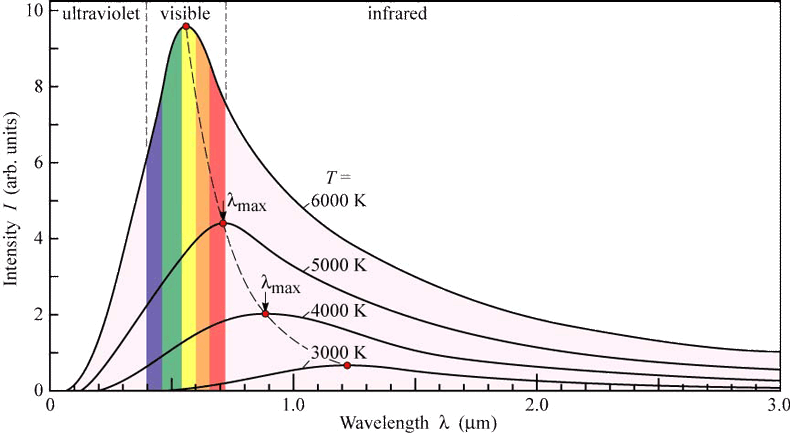
\includegraphics[width=0.5\linewidth]{wiendisplacement.png}
    \caption{The intensity vs wavelength plots, showing the Wien's displacement law.}
    \label{fig:wiendisplacement}
 \end{figure}

 Now, let us look at the origin of the Planck distribution. We start with the wave equation.
 \begin{equation}
    \frac{1}{s^2}\periv{^2y}{t^2}=\periv{^2y}{x^2}
 \end{equation}
 Solutions to this equation are either plane waves,
 \begin{equation}
    y_k(x,t) = A\sin kxe^{-i\omega t} \implies \frac{1}{s^2}\omega^2\ddot{y}_k = k^2y_K
 \end{equation}
 or harmonic oscillators with energies
 \begin{equation}
    \varepsilon_n = \lrp{n+\frac{1}{2}}\hbar\omega(k).
 \end{equation}
 The harmonic oscillator solution introduces packets of energy quantised by an integer number $n$. These quanta of energy were later named photons. The introduction of photons forms the foundation of quantum mechanics. \\
 Now we calculate the average number of particles with wavevector $\v{k}$ and energy $\hbar\omega(\v{k})$.
 \begin{equation}
    \bar{n}(\v{k}) = \sum_n^\infty np_n(\v{k})=\sum_n^\infty n\frac{e^{-n\beta\hbar\omega(\v{k})}}{Z(\v{k})}
    \label{eq:planckdist}
 \end{equation}
 Assuming isotropic distribution,
\begin{align}
    Z(k) =& 1 + \underbrace{e^{-\beta\hbar\omega}}_\text{1 photon} + \underbrace{e^{-2\hbar\omega\beta}}_\text{2 photons} + ... \notag\\
    =& \sum_n^\infty e^{-n\beta\hbar\omega(k)} = \frac{1}{1-e^{-\beta\hbar\omega(k)}}. 
    \label{eq:planckpartition}
\end{align}
Substituting (\ref{eq:planckpartition}) in (\ref{eq:planckdist}),
\begin{align}
    \bar{n} =& \sum_n^\infty ne^{-n\beta\hbar\omega(k)}\lrp{1-e^{-\beta\hbar\omega(k)}} = \lrp{1-e^{-\beta\hbar\omega(k)}}\sum_n^\infty  ne^{-n\beta\hbar\omega(k)} \notag\\
            =& -\lrp{1-e^{-\beta\hbar\omega(k)}}\periv{}{(\beta\hbar\omega)}\sum_n^\infty e^{-n\beta\hbar\omega(k)}\notag\\
            =& -\lrp{1-e^{-\beta\hbar\omega(k)}}\periv{}{(\beta\hbar\omega)}\lrp{\frac{1}{1-e^{-\beta\hbar\omega(k)}}}\notag\\
            =& (1-e^{-\beta\hbar\omega(k)})\frac{e^{-\beta\hbar\omega(k)}}{(1-e^{-\beta\hbar\omega(k)})^2} = \frac{e^{-\beta\hbar\omega(k)}}{1-e^{-\beta\hbar\omega(k)}}
\end{align}
\begin{equation}
    \therefore \bar{n}=\frac{1}{e^{\beta\hbar\omega(k)}-1}\implies \bar{u}(\v{k}) = \hbar\omega(k)\bar{n}(\v{k})
\end{equation}
Remember that, 
\begin{equation}
    u(\lambda) = D(\lambda)\frac{E(\lambda)}{V} = \frac{8\pi V}{\lambda^4}\hbar\omega(k)\frac{1}{e^{\beta\hbar\omega}-1}\frac{1}{V}.
\end{equation}
Also, $\hbar\omega(k) = \hbar ck = \hbar c\frac{2\pi}{\lambda}=\frac{hc}{\lambda}$. Putting everything together, we get the Planck distribution.
\begin{equation}
    u(\lambda) = \frac{8\pi}{\lambda^5}\frac{hc}{e^{\beta\hbar c/\lambda}-1}
\end{equation}
\begin{figure}[h!]
   \centering
   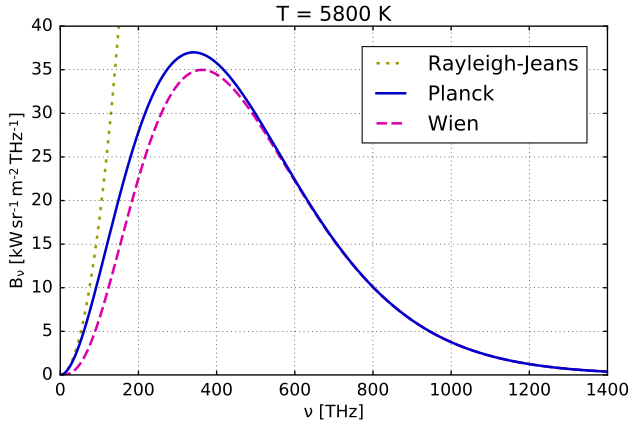
\includegraphics[width=0.5\linewidth]{blackbodydist.png}
   \caption{Three approaches to explain the black body spectra.}
   \label{fig:blackbodydist}
\end{figure}
\newpage

\section{Thermodynamics of the \\
Planck Distribution}
    The electromagnetic waves with different wavelengths in the cavity are distinguishable. Then, we can factorise the partition function. 
    \begin{equation}
        Z = Z(\v{k}_1)Z(\v{k}_2)...
    \end{equation}

    Looking at the Helmholtz free energy,
    \begin{equation}
        F = -k_BT\ln Z = -k_BT\sum_i\ln Z(\v{k}_i).
    \end{equation}
    If the distribution is isotropic, the sum can be written as the integral
    \begin{equation}
        F \approx -k_BT\int dk D(k)\ln Z(k).
    \end{equation}
    If we consider only the integral,
    \begin{equation}
        I = -2\frac{V}{2\pi^2}\int_{0}^{\infty}k^2\ln(1-e^{\beta\hbar ck})dk).
    \end{equation}
    Let us do a change of variables $x=\beta\hbar ck$ and use integration by parts.
    \begin{equation}
        I = -\frac{V}{\pi^2}\lrp{\frac{1}{\beta\hbar c}}^3\int_{0}^{\infty}x^2\ln(1-e^{-x})dx
    \end{equation}
    \begin{equation}
        \begin{rcases}
            x^2dx = dv ,\hspace{0.25cm} \frac{x^3}{3}=v\\
            u = (1-e^{-x} ),\hspace{0.25cm} du = \frac{dx}{e^x-1}
        \end{rcases} \Rightarrow I = \frac{-V}{\pi^2}\lrp{\frac{k_BT}{\hbar c}^3}\lrb{\underbrace{\lrp{\frac{x^3}{3}(1-e^{-x})}_0^\infty}_0 - \underbrace{\int_{0}^{\infty}\frac{x^3}{3}\frac{dx}{e^x-1}}_{\pi^4/15}}\notag
    \end{equation}
    \begin{equation}
         = \frac{V}{3\pi^2}\lrp{\frac{k_BT}{\hbar c}}^3\frac{\pi^4}{15}
    \end{equation}
    \begin{align}
        F =& -k_BTI=-\frac{\pi^2V}{45}\frac{(k_BT)^4}{(\hbar c)^3}\equiv -AT^4\\
        S =& -\periv{F}{T}=4AT^3\\
        P =& -\periv{F}{V}=\frac{AT^4}{V} \\
        U =& F+TS=3AT^4
    \end{align}
    Looking at the internal energy and the pressure, we see that
    \begin{equation}
        U =3PV.
    \end{equation}
    The source of this pressure is the momenta imparted by the photons on the walls of the cavity.

\section{Einstein's Model of Vibrations in Solids}
    The idea of quantization can be extended to matter waves as well as demonstrated by de Broglie in his PhD thesis. Consider the highly ordered atoms in a crystal. Let $x_i^0$ denote the positions of the lattice points of the crystal and $u_i$ the deviation of the positions of the atoms in the crystal as they vibrate. The internal energy is a function of these positions.
    \begin{equation}
        U = U(x_i^0+u_i)
    \end{equation}
    Considering the vibrations as small oscillations, we can Taylor expand this expression around the equilibrium points, i.e. the lattice points. 
    \begin{equation}
        U = U_0 +\sum_i^N \periv{U}{x_i}\bigg\vert_{x_i=x_i^0}u_i + \frac{1}{2}\sum_{i,j}^N\periv{^2U}{x_i\del x_j}u_iu_j+...
    \end{equation}
    Here, we can ignore the constant term $U_0$ and neglect the first sum. Moreover, we can define $K_{ij}=\del_i\del_jU$ to get the internal energy as a generalised harmonic oscillator.
    \begin{equation}
        U = \sum_{ij}^N\frac{1}{2}K_{ij}u_iu_j
    \end{equation}
    In this approximation, the vibration modes can be treated as quanta of energy with
    \begin{equation}
        Z = \frac{1}{1-e^{\beta\hbar\omega}}.
    \end{equation}
    Then, the free energy for N oscillators is 
    \begin{equation}
        F = k_BT\sum_\alpha \ln(1-e^{\beta\hbar\omega_\alpha})
    \end{equation}
    where we sum over all the modes of vibration. Moreover, we can add a term representing the zero point energy of the oscillations and the energy of interactions between atoms in their equilibrium positions. This gives us 
    \begin{equation}
        F = N\epsilon + k_BT\sum_\alpha \ln(1-e^{-\beta\hbar\omega_\alpha}).
        \label{eq:einsteinfreeenergy}
    \end{equation}
    \paragraph{Einstein's model of vibrations:}All modes of vibration have the same angular frequency $\omega_E$. Therefore, each mode has energy $\hbar\omega_E$. Then the sum in (\ref{eq:einsteinfreeenergy}) just gives $3Nk_BT\ln(...)$. The Helmholtz free energy is thus
    \begin{equation}
        F = N\epsilon + 3Nk_BT\ln(1-e^{-\beta\hbar\omega_E}).
        \label{eq:einsteinfreeenergy2}
    \end{equation}
    Taking the second derivative of this twice and multiplying by $(-T)$ gives us the heat capacity.
    \begin{equation}
        C_V = 3Nk_B\frac{(\beta\hbar\omega_E)^2e^{\beta\hbar\omega_E}}{(e^{\beta\hbar\omega}-1)^2}
    \end{equation}
    At high temperatures, the exponential is small. Thus, we can expand it in Taylor series. For $x=\beta\hbar\omega_E$,
    \begin{equation}
        C_V\approx ^Nk_Bx^2\frac{1+x+\frac{x^2}{2}+...}{(1+x-1)^2}\approx ^Nk_B\frac{x^2}{x^2}=3Nk_B.
    \end{equation}
    Moreover, at low temperatures, $x>>1$. 
    \begin{equation}
        C_V\approx 3Nk_Bx^2\frac{e^x}{(e^x-1)^2}=\frac{3NkBx^2e^x}{e^{2x}}=3NkB\lrp{\frac{\hbar\omega_E}{k_BT}}^2e^{-\hbar\omega_E/k_BT}
    \end{equation}
    This model fits the experiment well for high temperatures but fails at very low temperatures. 

\section{Debye's Model of Vibrations in Solids}
    Debye's model is an improvement over Einstein's model, where temperature ranges are treated separately. This helps fix the deviations of the model from the experimental data at low temperatures. At low temperatures, i.e. long wavelengths, acoustic waves are highly populated where there are many atoms per wavelength. In contrast, at hight temperatures with short wavelengths, the optical waves are populated. This proposes a wavelength dependence on the frequency of vibrations. We know this functional dependence of $\omega$ on $k$ as the \textbf{dispersion relation}. \\
    In three dimensions, for each $\lambda$, there are three modes of vibration, i.e. polarizations: Two transverse and one longitudinal mode per wavelength. \\
    For the thermodynamic properties, we start with the density of states. Since the wavevectors are discretised in exactly the same way as it was for an ideal gas, we can use the same formula for the density of states in the $k$-space. For a single polarization, 
    \begin{equation}
        D(k)dk = \frac{Vk^2dk}{2\pi^2}.
    \end{equation}
    Now, we convert the density of states to an expression in terms of the angular frequency. The transverse and longitudinal waves, in general, have different speeds for acoustic waves: $\omega_L=s_Lk$ and $\omega_T=s_Tk$. However, both are linear in wavenumber. Thus, let us derive $D(\omega)$ for a generic speed $s$. 
    \begin{equation}
        \omega = sk \implies k =\frac{\omega}{s}
    \end{equation}
    \begin{equation}
        D(\omega)=D(k(\omega))\deriv{k}{\omega}=\frac{Vk^2}{2\pi^2}\frac{1}{s}=\frac{V(\omega/s)^2}{2\pi^2s}=V\frac{\omega^2}{2\pi^2s^3}
    \end{equation}
    Now, we add all three contributions. Two from $s_T$ and one from $s_L$.\footnote{These also give the average speed of sound as $\frac{3}{\bar{s}^3}=\frac{2}{s_T^3}+\frac{1}{s_L^3}$.}
    \begin{equation}
        D(\omega) = \frac{V\omega^2}{2\pi^2}\lrp{\frac{2}{s_T^3}+\frac{1}{s_L^3}}
    \end{equation}
    In Debye's model, this density of states is used to calculate the Helmholtz free energy for acoustic waves. At low temperatures (or large frequencies), free energy is again a sum that we can write using an integral.
    \begin{equation}
        F \approx N\epsilon + \int_0^{2\pi s/\lambda_\text{min}} D(\omega)\ln(1-e^{\hbar\omega\beta})d\omega =\footnote{Since $\lambda_\text{min}\approx a$ where $a$ is a lattice constraint, it can be represented by an infinity} N\epsilon + \frac{3k_BTV}{2\pi^2\bar{s}^3}\int_{0}^{\infty}\omega^2\ln(1-e^{-\hbar\omega\beta})d\omega
    \end{equation}
    Using integration by parts and utilising the $\Gamma-$function, this integral gives
    \begin{equation}
        F = N\epsilon - \frac{\pi^2k_B^4T^4V}{30\hbar^3\bar{s}^3}
    \end{equation}
    with entropy as
    \begin{equation}
        S = \frac{2\pi^2k_B^4V}{15\hbar^3\bar{s}^3}T^3
    \end{equation}
    Now, for high temperatures (or small frequencies)
    \begin{align}
        F =& N\epsilon + k_BT\sum_\alpha \ln(1-e^{-\hbar\omega_a/k_BT})\approx N\epsilon + k_BT\sum_\alpha \ln\lrp{1-1+\frac{\hbar\omega_\alpha}{k_BT}}\notag \\
        =&N\epsilon + k_BT\sum_\alpha\ln\lrp{\frac{\hbar\omega_\alpha}{k_BT}} = N\epsilon + 3Nk_BT\ln\lrp{\frac{\hbar}{k_BT}}+k_BT\sum_\alpha\ln\omega_\alpha
    \end{align}
    We can define an average frequency by 
    \begin{equation}
        \ln\bar{\omega} = \frac{1}{3N}\sum_\alpha\ln\omega_\alpha.
    \end{equation}
    Then, 
    \begin{equation}
        F = N\epsilon + 3Nk_BT\ln\frac{\hbar}{k_BT}+3Nk_BT\ln\bar{\omega}
    \end{equation}
    Then we get $F\propto 3Nk_BT\ln AT$ which gives $C_V = 3Nk_B$. This is consistent with the equipartiton theorem. \\
    So far, we've been distinguishing the long and short wavelengths, high and low temperatures, large and small frequencies, etc. So, a natural question is: What is the cutoff frequency such that the long and short wavelengths can be distinguished? Or similarly, high temperature and low temperature? Here, we introduce the \textbf{Debye frequency} $\omega_D$ chosen so that the number of modes up to $\omega_D$ is $3N$. We then interpolate between the two regimes. 
    \begin{equation}
        3N = \int_{0}^{\omega_D}D(\omega)d\omega = \frac{3V}{2\pi^2\bar{s}^3}\int_{0}^{\omega_D}\omega^2d\omega = \frac{V\omega_D^3}{2\pi^2\bar{s}^3}
    \end{equation}
    \begin{equation}
        \implies \omega_D = \bar{s}\lrp{\frac{6N\pi^2}{V}}^{1/3}=\bar{s}\lrp{6n\pi^2}^{1/3}
    \end{equation}
    Using $\omega_D$ we can also define a \textbf{Debye energy} $\hbar\omega_D$ and a \textbf{Debye temperature} $T_D=\hbar\omega_D/k_B$. This Debye temperature is considered a border between high temperature and low temperature. In the Debye theory,
    \begin{equation}
        D(\omega)=\begin{cases}
            \frac{3V}{2\pi^2\bar{s}^3}\omega^2, & \omega<\omega_D \\
            0, & \omega>\omega_D
        \end{cases}
    \end{equation}
    Then,
    \begin{equation}
        F = N\epsilon + \frac{3k_BTV}{2\pi^2\bar{s}^3}\lrp{\frac{k_BT}{\hbar}}^3\int_{0}^{\hbar\omega_D/k_BT}x^2\ln(1-e^{-x})dx.
    \end{equation}
    As examples, the Debye temperature for Silicon is $647K$ while for Potassium, it is $89.4K$. One weak side of the Debye theory is that at very low temperatures, $C_V$ is still not consistent with the expermiental results due to electronic degrees of freedom that are not accounted by the Debye model. 
\section{Solids and Vapours in Equilibrium}
    Until now, we have seen how to calculate the partition functions for solids and gases. With this knowledge, we can look for a theory on the equilibrium between these phases knowing that at equilibrium, the Helmholtz free energy is minimised. For simplicity, we will take the gas to be Argon since it is monoatomic and spinless and use Einstein's theory for the solid. The interactions between the gas and the solid are taken to be weak so that the total partition function can be factorised into a product of the partition functions of each phases. The partition function for a solid with $N_S$ atoms can be derived from (\ref{eq:einsteinfreeenergy2}). Multiplying the first term by unity,
    \begin{align}
        F =& k_BT\beta N_S\epsilon + 3N_Sk_BT\ln(1-e^{-\beta\hbar\omega}) = k_BT\lrp{\beta N_S\epsilon + 3N_S\ln(1-e^{-\beta\hbar\omega})} \notag\\
          =& k_BT\lrp{\ln e^{\beta N_S\epsilon}+\ln(1-e^{-\beta\hbar\omega})^{3N}} = k_BT\ln\lrb{e^{\beta N_S\epsilon}(1-e^{-\beta\hbar\omega})^{3N}}
    \end{align}
    \begin{equation}
        \therefore Z_S = e^{-N_S\epsilon/k_BT}\lrp{\frac{1}{1-e^{-\hbar\omega_E/k_BT}}}^{3N}
    \end{equation}
    Here, $-\epsilon$ is the energy per atom needed to break the solid apart into seperate gas atoms and $\omega_E$ is the Einstein frequency of vibration.\\
    We know that the partition function of the gas is
    \begin{equation}
        Z_G = \frac{Z_1^{N_G}}{N_G!}
    \end{equation}
    where $Z_1$ is the single particle partition function of the gas atom. Since the gas is monoatomic and spinless, only contribution to the partition function is from the translational motion of the atoms. As we stated before, the total partition function is
    \begin{equation}
        Z = Z_GZ_S
    \end{equation}
    When an atom leaves the solid and becomes a vapour, the total number of particles does not change. Thus, $N_G+N_S$ is constant and $dN_G=-dN_S$. From the partition function, the free energy is
    \begin{equation}
        F = -k_BT\ln Z_S -k_BT\ln Z_G
    \end{equation}
    By minimising this expression as a function of $N_G$, we get
    \begin{equation}
        \periv{F}{N_G} = k_BT\periv{\ln Z_S}{N_S}-k_BT\periv{\ln Z_G}{N_G}=0.
    \end{equation}
    After some algebra, 
    \begin{equation}
        \frac{Z_1}{N_G} = \frac{e^{-\epsilon/k_BT}}{(1-e^{-\hbar\omega_E/k_BT})^3}
    \end{equation}
    By using the ideal gas law, $P=N_Gk_BT/V_G$ where $V_G$ is the volume of the gas, we get
    \begin{equation}
        P = \frac{k_BTZ_1}{V_G}e^{\epsilon/k_BT}(1-e^{-\hbar\omega_E/k_BT})^3.
    \end{equation}
    This is very crude model for the mechanics of a solid. To further improve it, we can use the Debye's model rather than Einstein's, take into account the effects of vacancies left by the atoms leaving the solid, consider a more general case with spin and take the entropy contribution into account, and include rotational and vibrational effects of a molecule into $Z_G$. 